\documentclass[%
	%draft
	]{ijsra}
\def\IJSRAidentifier{\currfilebase} %<---- don’t change this!
%-------Title | Email | Keywords | Abstract-------------
\def\shorttitle{Neolithic and Early Bronze Age Research Student Symposium}
\def\maintitle{The \nth{3} Neolithic and Early Bronze Age Research Student Symposium,\\ University College London: Institute of Archaeology}
\def\cmail{tcrnbgh@ucl.ac.uk}
%\def\keywords{Research, Archaeology, ...}
%\def\keywordname{}%<--- redefine the name “Keywords“ in needed language
%\def\abstract{In their paper Jon and Jon are showing ...}
%--------Author’s names------------
\def\authorone{Barney Harris}
\def\authortwo{Dannielle Croucher}
\def\authorthree{Hayden McKee}
%\def\authorfour{}%<---- comment or delete if you do not need a fourth author.
%\def\authorfive{}%<---- comment or delete if you do not need a fifth author.
%-------Biographical information-------------
\def\bioone{Barney Harris is a doctoral student at UCL's Institute of Archaeology (IOA) where he researches monumental construction in Neolithic Wessex.}
\def\biotwo{Danielle Croucher is a MSc student at UCL's Institute of Archaeology, studying archaeologicla skeletal remains.}%<---- comment or delete if there is no second author.
\def\biothree{Hayden McKee is also a MSc student at UCL's Institute of Archaeology, studying archaeologicla skeletal remains.}%<---- comment or delete if there is no third author.
%\def\biofour{}%<---- comment or delete if there is no fourth author.
%\def\biofive{}%<---- comment or delete if there is no fifth author.
%------University/Institution--------------
\def\affilone{†‡University College London, Institute of Archaeology}
%\def\affiltwo{University College London, Institute of Archaeology}%<---- comment or delete if there is no second author.
%\def\affilthree{University College London, Institute of Archaeology}%<---- comment or delete if there is no third author.
%\def\affilfour{}%<---- comment or delete if there is no fourth author.
%\def\affilfive{}%<---- comment or delete if there is no fifth author.
%--------Mapping of authors to affiliations------------
%% authorone:--> * <--- copy/paste that symbol to \affiloneauthor etc. below
%% authortwo:--> † <--- copy/paste that symbol to \affiloneauthor etc. below
%% authorthree:--> ‡ <--- copy/paste that symbol to \affiloneauthor etc. below
%% authorfour: --> § <--- copy/paste that symbol to \affiloneauthor etc. below
%% authorfive: --> ¶ <--- copy/paste that symbol to \affiloneauthor etc. below
%-------------------------------------------------------------------------
\def\affiloneauthor{*}%<---- paste the symbol of the authors into {}
\def\affiltwoauthor{†}%<---- paste the symbol of the authors into {}
\def\affilthreeauthor{‡}%<---- paste the symbol of the authors into {}
%\def\affilfourauthor{}%<---- paste the symbol of the authors into {}
%\def\affilfiveauthor{}%<---- paste the symbol of the authors into {}

\begin{filecontents}{\IJSRAidentifier.bib}
%Bibliography-data HERE
\end{filecontents}
\IJSRAopening
%-------
\lettrine{T}{he} \nth{3} annual Neolithic and Early Bronze Age Research Student Symposium (NEBARSS) took place on the 18th and 19th of November 2016 at the UCL Institute of Archaeology in London (Fig. \ref{fig:34-Harris-figure02}). The 2016 symposium followed previous NEBARSS events at Newcastle University (2015) and the University of Bradford (2014). Speakers at the 2016 symposium discussed a broad range of archaeological research into the Neolithic and Early Bronze Age periods and the event provided a platform for postgraduate, independent and early career researchers to present their work in an informal environment. The symposium was organised by PhD students Barney Harris and Robert Kaleta and was kindly sponsored by the Prehistoric Society and the UCL Joint Faculty Institute of Graduate Studies.

%Figure 1 needs caption and links in text

\begin{figure}[!htb]
	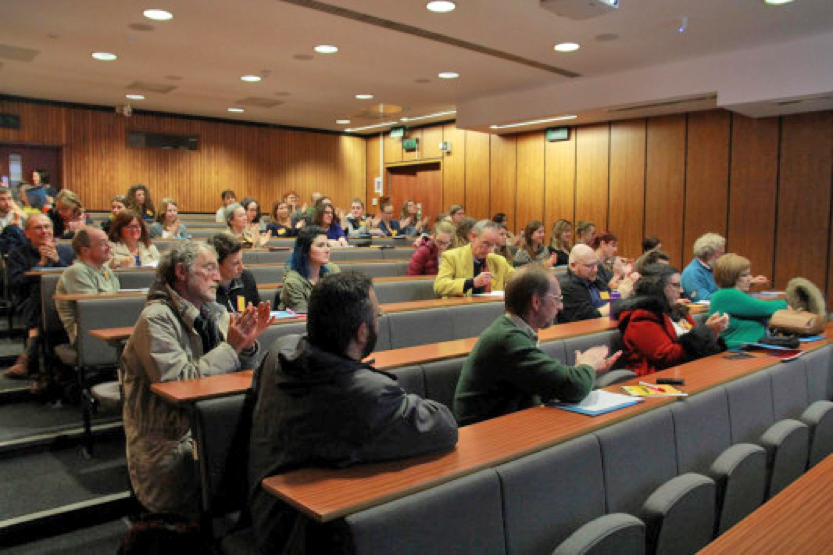
\includegraphics[width=\linewidth]{34-Harris-figure01}
	\caption{Attendees at the \nth{3} annual Neolithic and Early Bronze Age Research Student Symposium (NEBARSS)
		{\normalfont\scriptsize \\ \copyright\ by \shortauthor
	}}
	\label{fig:34-Harris-figure01}
\end{figure}

The theme of the 2016 symposium was ‘\textit{anarchy in the UK?}anarchy in the UK?’, a playful concept designed to challenge speakers to consider how their work contributes to understanding social change in prehistory beyond linear, evolutionary narratives of increasing hierarchical control. The theme also highlighted the importance of revolutionary shifts within archaeological theory. 

The conference commenced on the evening of Friday \nth{18}, with a keynote lecture from University College London’s Professor Mike Parker Pearson. His presentation, ‘\textit{Back to the future: contemporary issues in British later prehistory}’, 
highlighted an emerging new scientific era in archaeology based on Big Data, quantitative modelling, materiality studies, Actor Network Theory, ancient DNA and isotope analyses. His own research on the genetics of Neolithic Bell Beaker communities demonstrated the potential for new analytical technologies to contribute to research questions framed by post-processual archaeological theory. The lecture was followed by questions and a wine reception (Fig. \ref{fig:34-Harris-figure02}). 


%Figure 2 needs caption and links in text

\begin{figure}[!htb]
	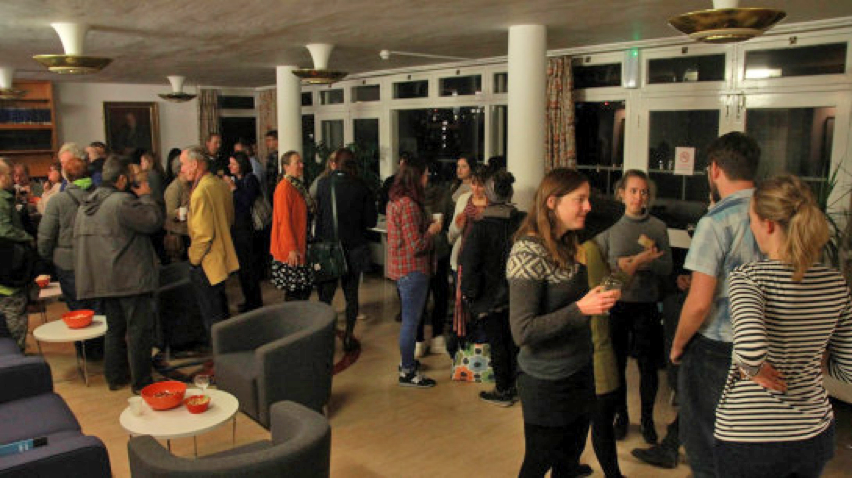
\includegraphics[width=\linewidth]{34-Harris-figure02}
	\caption{Wine reception at the \nth{3} annual Neolithic and Early Bronze Age Research Student Symposium (NEBARSS)
		{\normalfont\scriptsize \\ \copyright\ by \shortauthor
	}}
	\label{fig:34-Harris-figure02}
\end{figure}


On Saturday the \nth{19} the first session included new research on challenging the connotations of animal domesticity (Emily Banfield, University of Leicester), visualisation of Neolithic domestic dwellings in the Milfield Basin (Seren Griffiths, University of Central Lancashire) and domestication of Neolithic-Bronze Age mind (Alexander Aston, University of Oxford). The second session centred on monumental construction and labour, including papers on the origins of the sarsen stones at Stonehenge (Katy Whitaker, University of Reading), the construction of communities through long barrow building, reviewed through assemblage theory (Mareike Ahlers, Newcastle University) and a review of Renfrew’s (in)famous chiefdom hypothesis in light of additional labour estimates for  monumental construction in Wessex (Barney Harris, UCL Institute of Archaeology).

The third session included talks on the significance of categorising artefacts, using the Unstan Bowl as a case study (Michael Copper, University of Bradford), farming and ceramic production in Anatolia (Beatrijs De Groot, UCL Institute of Archaeology) and highlighting the alleged absence of cremations in the British Chalcolithic funerary record (Anna Bloxam, UCL Institute of Archaeology). The fourth and final session focused on emerging digital platforms for engaging the public in archaeological sites and centred around a current project at Ҫatalhöyük, Turkey (Tara Copplestone and Izzy Bartley, University of York and University of Aarhus), the reoccurring colours, red, black and white in the Neolithic megalithic monuments of Atlantic Europe (Penelope Foreman, Bournemouth University) and concluded with a second keynote lecture from Dr. Joanna Brück on mortuary practices and social evolution in Early and Middle Bronze Age Britain, with a critical reevaluation of the Amesbury Archer and the Boscombe Bowmen burials.

The symposium created a relaxed and safe environment for new researchers to gain experience in presentation, promote current research and gain valuable insights from other academics, as well as providing a highly captivating day of archaeological research for the audience. The environment was positive and encouraging form all guests, volunteers, speakers and professors, and we look forward to next year’s symposium hosted at the University of Central Lancashire (UCLAN).


\IJSRAclosing